\section{First approach: KG-based IR system}

\begin{frame}{Experiments objective}

    \begin{center}
        From a text-based to a concept-based search.
    \end{center}

    \begin{figure} [H]
        \begin{center}
            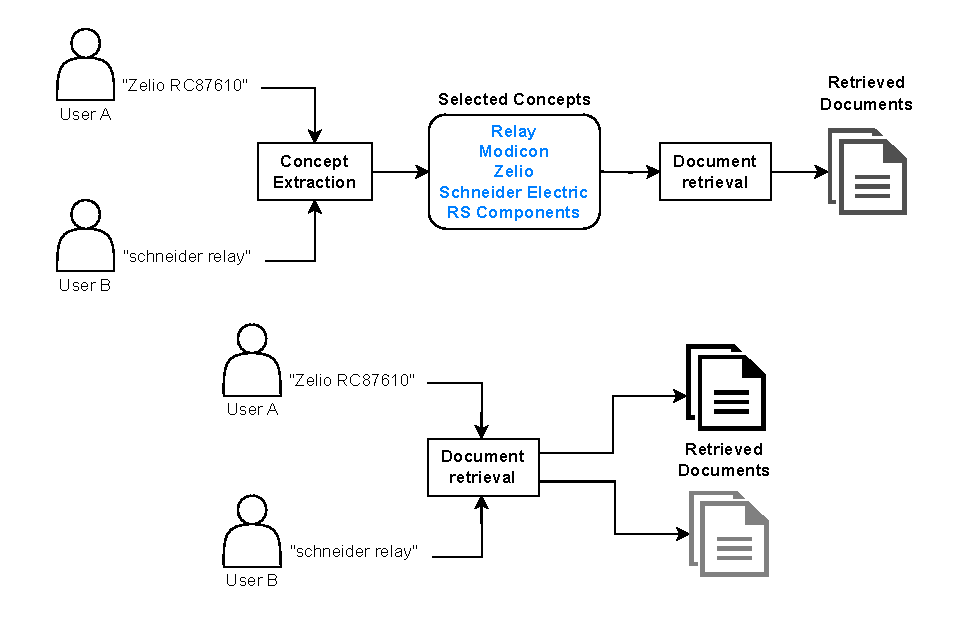
\includegraphics[scale=0.6]{images/text-vs-concept-based-search.pdf} 
            \caption{Text-based vs concept-based search.} 
        \end{center}
    \end{figure}

\end{frame}

\begin{frame}{Experiments protocol}

    \begin{figure} [H]
        \begin{center}
            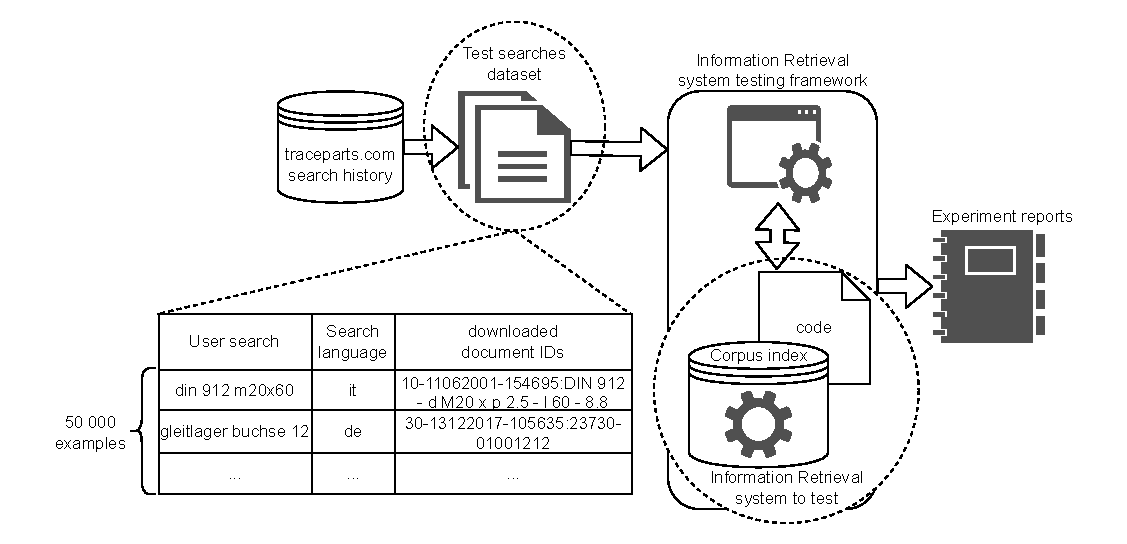
\includegraphics[scale=0.6]{images/tp-search-expe-setting.pdf} 
            \caption{Experiments Protocol.} 
        \end{center}
    \end{figure}

\end{frame}

\begin{frame}{Evaluation metrics}

    \begin{itemize}
        \item Mean Average Precision at k (MAP@k): 
        \begin{itemize}
            \item A sliding (or growing) precision window, averaged over a set of query examples.
            \item Ranges from $0$ to $1$ ($1$ is the best value).
            \item Gives information about the amount and positions of positive results in the k first ones.
        \end{itemize}
        \item Binary Mean at k (BM@k):
        \begin{itemize}
            \item Binary average over a set of query examples.
            \item Ranges from $0$ to $1$ ($1$ is the best value).
            \item Provides information about the amount of queries with a positive result in the k first ones.
            \item Does not give any detail on the positive result position.
        \end{itemize}
    \end{itemize}

\end{frame}

\begin{frame}{Information Retrieval systems}

    6 distinct systems built iteratively:
    \begin{itemize}
        \item Text-based system (baseline)
        \item Concept-based system
        \item Knowledge Graph-based system
        \item Text-based system with implicit knowledge
        \item Concept-based system with implicit knowledge
        \item Knowledge Graph-based system with implicit knowledge
    \end{itemize}

    Implementation:
    \begin{itemize}
        \item User search concept matching problem as an information retrieval task.
        \item Leverage user search history as implicit knowledge.
        \item Query concept enrichment as a graph traversal task.
    \end{itemize}

\end{frame}

\begin{frame}{Information Retrieval systems}

    \begin{figure} [H]
        \begin{center}
            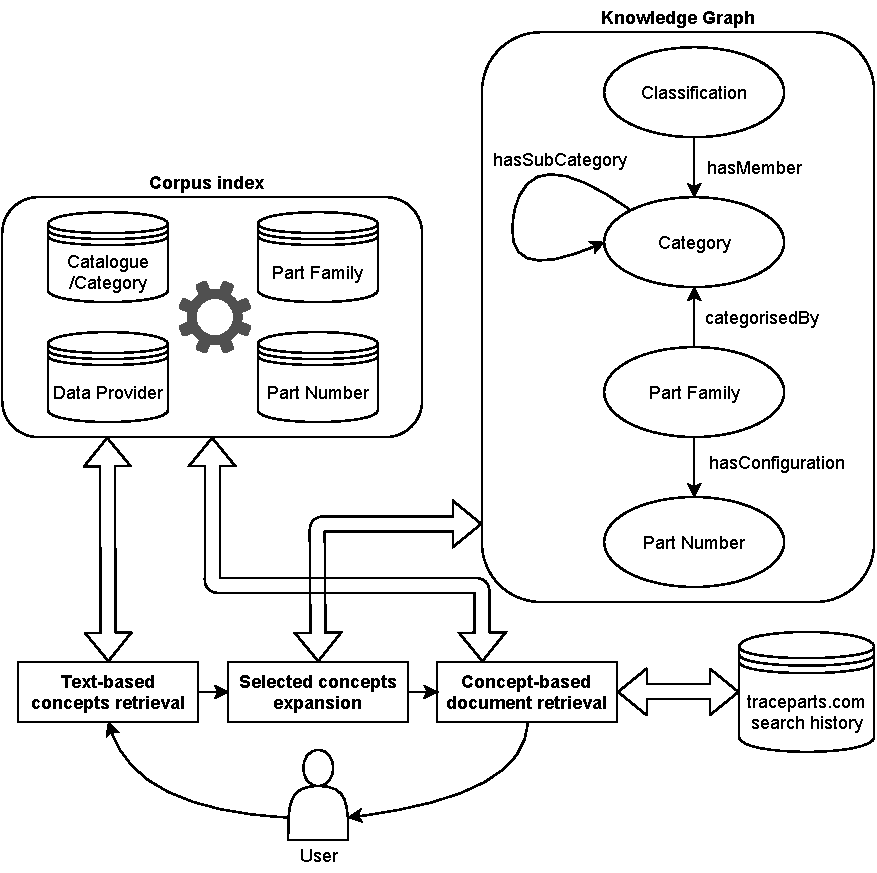
\includegraphics[scale=0.45]{images/kg-based-ir-system-with-search-hist.pdf} 
            \caption{Knowledge Graph-based system with implicit knowledge.} 
        \end{center}
    \end{figure}

\end{frame}


\begin{frame}{Results}

    \begin{table}[htbp]
        \begin{center}
        \small
        \begin{tabular}{c|cc|cc|cc|}
            \toprule
            \multicolumn{1}{l}{}               & \multicolumn{2}{c}{\textbf{\begin{tabular}[c]{@{}c@{}}Text-based\\ system (baseline)\end{tabular}}}  & \multicolumn{2}{c}{\textbf{\begin{tabular}[c]{@{}c@{}}Concept-based\\ system\end{tabular}}} & \multicolumn{2}{c}{\textbf{\begin{tabular}[c]{@{}c@{}}KG-based system\\with search history\end{tabular}}} \\ \cmidrule(lr){2-7} %\cmidrule(lr){2-4}\cmidrule(lr){5-7}\cmidrule(lr){8-10}
            \multicolumn{1}{c|}{\textbf{@k $\downarrow$}}    & \multicolumn{1}{c}{\textbf{MAP@k}}  & \textbf{BM@k} & \multicolumn{1}{|c}{\textbf{MAP@k}} & \textbf{BM@k}  & \multicolumn{1}{|c}{\textbf{MAP@k}} & \textbf{BM@k} \\ \cmidrule(lr){2-7}
            \multicolumn{1}{c|}{\textbf{@5}}   & \multicolumn{1}{c}{0.061}          & 0.114         & \multicolumn{1}{|c}{0.152} & 0.243 & \multicolumn{1}{|c}{0.115}          & \textbf{0.291}        \\ 
            \multicolumn{1}{c|}{\textbf{@25}}  & \multicolumn{1}{c}{0.064}          & 0.148         & \multicolumn{1}{|c}{0.159} & 0.334 & \multicolumn{1}{|c}{0.122}          & \textbf{0.471}         \\ 
            \multicolumn{1}{c|}{\textbf{@50}}  & \multicolumn{1}{c}{0.064}          & 0.157         & \multicolumn{1}{|c}{0.160} & 0.371 & \multicolumn{1}{|c}{0.123}          & \textbf{0.552}         \\ 
            \multicolumn{1}{c|}{\textbf{@100}} & \multicolumn{1}{c}{0.064}          & 0.161         & \multicolumn{1}{|c}{0.161} & 0.403 & \multicolumn{1}{|c}{0.123}          & \textbf{0.624}         \\ 
            \multicolumn{1}{c|}{\textbf{@350}} & \multicolumn{1}{c}{0.064}          & 0.164         & \multicolumn{1}{|c}{0.161} & 0.429 & \multicolumn{1}{|c}{0.124}          & \textbf{0.715}         \\ \bottomrule
        \end{tabular}
        \caption{
            Comparing text, concept, and KG-based systems for different k values.
        }\label{tab:comp-text-concept-kg}
    \end{center}
    \end{table} 

\end{frame}

\begin{frame}{Results}

    \begin{table}[htbp]
        \begin{center}
        \small
        \begin{tabular}{ccc}
            \toprule
            {} &  \textbf{No results}  &  \textbf{\begin{tabular}[c]{@{}c@{}}Less than 400\\ results (non empty)\end{tabular}} \\
            \midrule
            \textbf{\begin{tabular}[c]{@{}c@{}}Text-based\\ system (baseline)\end{tabular}}              &     64.48\% &              35.44\% \\
            \textbf{\begin{tabular}[c]{@{}c@{}}Concept-based\\ system\end{tabular}}                      &     11.43\% &              \textbf{88.36\%} \\
            \textbf{\begin{tabular}[c]{@{}c@{}}KG-based system\\with search history\end{tabular}}      &     \textbf{8.10\%} &       51.59\% \\
            \bottomrule
        \end{tabular}
        \caption{
            Comparing all search systems results set corpus.
        }\label{tab:comp-all-sys-res-list}
    \end{center}
    \end{table}

\end{frame}